\chapter{Double Scenario Classification of the last shared app, KFold Validation}Starting with fitting randomly the classifiers, there are some statistics of the data used for the first test: \\
 {\def\arraystretch{1.3} 
 \begin{table}[H] 
\centering 
\begin{tabular}{|l|l|l|} 
\hline 
  &count train  &count test  \\ \hline
messenger  &302  &748  \\ \hline
telegram  &314  &736  \\ \hline
whatsapp  &340  &710  \\ \hline
original  &94  &256  \\ \hline
\end{tabular} 
\end{table} }
\section{Logistic regression results:} 
Confusion matrix with number of sample and with normalization:
 {\def\arraystretch{1.3} 
 \begin{table}[H] 
\centering 
\begin{tabular}{|l|l|l|l|l|} 
\hline 
  &messenger  &telegram  &whatsapp  &original  \\ \hline
messenger  &746  &0  &2  &0  \\ \hline
telegram  &0  &618  &118  &0  \\ \hline
whatsapp  &0  &216  &494  &0  \\ \hline
original  &0  &0  &8  &248  \\ \hline
\end{tabular} 
\end{table} }

 \begin{figure}[H] 
\centering 
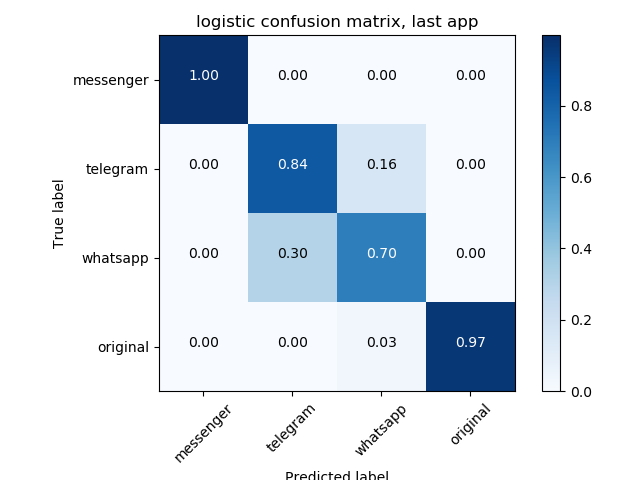
\includegraphics[scale=.6]{images/new_met_lr_initial_double_simple.png} 
\caption{logistic regression, last app classified} 
\end{figure} 


Result of the KFold validation with 10 bins: